% Use only LaTeX2e, calling the article.cls class and 12-point type.

\documentclass[11pt]{article}

\usepackage[round,semicolon]{natbib}
\usepackage{etoolbox}
\AtBeginEnvironment{quote}{\singlespacing\tiny}
% Use times if you have the font installed; otherwise, comment out the
% following line.

% added by SKH
%\usepackage{lineno}
%\linenumbers

\usepackage{times}
\usepackage{amssymb}
\usepackage{amsmath}

\usepackage[export]{adjustbox}

\usepackage{graphicx}
\graphicspath{ {images/} }

% for adjustwidth
\usepackage{changepage}

% The following parameters seem to provide a reasonable page setup.

\topmargin 0.0cm
\oddsidemargin 0.2cm
\textwidth 16cm 
\textheight 21cm
\footskip 1.0cm

\usepackage{newfloat}
\usepackage{amsmath}
\usepackage[labelfont=bf]{caption}
\usepackage{nameref}
\usepackage{rotating}
\usepackage{color}
\usepackage{float}
\renewcommand{\figurename}{{}}
\renewcommand{\thefigure}{{Figure \arabic{figure}}}

\renewcommand{\tablename}{{}}
\renewcommand{\thetable}{{Table \arabic{table}}}

\newfloat{suppfile}{thp}{losuppfile}
\renewcommand{\thesuppfile}{Supplementary file \arabic{suppfile}}
\floatname{suppfile}{}

\newfloat{suppfig}{thp}{losuppfig}
\renewcommand{\thesuppfig}{Supplementary figure \arabic{suppfig}}
\floatname{suppfig}{}

%
\newfloat{supptable}{thp}{losupptable}
\renewcommand{\thesupptable}{Supplementary table \arabic{supptable}}
\floatname{supptable}{}
%

\renewcommand{\theequation}{Equation \arabic{equation}}

\newcommand{\mutDNA}{\textbf{mutDNA}}
\newcommand{\mutvirus}{\textbf{mutvirus}}
\newcommand{\DNA}{\textbf{DNA}}
\newcommand{\virus}{\textbf{virus}}

\newcommand\skhcomment[1]{{\color{cyan}[#1]}}
\newcommand\jdbcomment[1]{{\color{red}[#1]}}


\usepackage{hyperref}
\hypersetup{colorlinks,citecolor=blue,linkcolor=blue,urlcolor=blue}
\hypersetup{colorlinks,citecolor=blue,linkcolor=blue,urlcolor=blue}

\usepackage{seqsplit}

\usepackage{array}
\newcolumntype{P}[1]{>{\raggedright\arraybackslash}p{#1}}

\title{Experimentally informed site-specific substitution models deepen phylogenetic estimates of the divergence of viral lineages} 

\author
{Sarah K. Hilton$^{1,2}$  and Jesse D. Bloom$^{1,2}$\\
\\
\normalsize{$^1$Division of Basic Sciences and Computational Biology Program,}\\
\normalsize{Fred Hutchinson Cancer Research Center, Seattle, WA 98109, USA}\\
\normalsize{$^2$Department of Genome Sciences, University of Washington, Seattle, WA}\\
\normalsize{E-mail:  jbloom@fredhutch.org.}\\
}


% Include the date command, but leave its argument blank.

\date{}

\usepackage{setspace}
\onehalfspacing


\begin{document} 

% Make the title.

\maketitle 


\begin{abstract}
\noindent  
Molecular phylogenetics is often used to estimate the time since the divergence of modern gene sequences.
Such phylogenetic techniques often estimate substantially shallower divergence times than other methods.
For instance, in the case of viruses there is independent evidence that molecular phylogenetics can underestimate deep divergence times.  
This discrepancy is thought to be caused in part by inadequate models of purifying selection leading to branch-length underestimation.
Here we show that substitution models informed by experimental measurements of the purifying selection due to site-specific amino-acid preferences lengthen the deep branches on phylogenies of influenza virus hemagglutinin.
This deepening of branch lengths is due to better modeling of the stationary state of the substitution models, and is independent of the branch-length-extension that results from modeling site-to-site variation in substitution rate.
The deepening of branch lengths from experimentally informed site-specific substitution models is similar to that achieved by other approaches that allow the stationary state to vary across sites.
However, the improvements from these site-specific models are limited by the inherent tension between the enhanced accuracy of accounting for site-specific amino-acid preferences and the fact that these preferences shift over long evolutionary times.
Overall, our work underscores the importance of modeling how site-specific purifying selection affects the stationary state when estimating deep divergence times. 
\end{abstract}

\clearpage

\section*{Introduction} 
\skhcomment{from JDB: what is the "age" of a virus? Maybe "divergence time of viral lineages"}
skhcomment{from JDB: what is the less than a million actually? "Old" is not the right phrase.}
Estimating the divergence time of viral lineages of a virus is essential to understanding its evolutionary history, including its emergence, spread, and past zoonoses. 
This estimation is commonly done using the concept a ``molecular clock" to transform the branch lengths of the viral phylogenetic tree into age in years. 
However, this molecular dating technique often underestimates the age of many viruses, including measles, foamy virus, and ebola \skhcomment{(citations)}, compared to other methods which are independent of the viral phylogeny. 
For example, SIV (the original source of HIV) is estimated to be less than a million years old based on the viral phylogeny \citep{sharp2000origins,wertheim2009dating,worobey2010island} but estimated to be several million years old based on the host tree or endogenous retroviral elements  \citep{compton2013host} \skhcomment{(other citations)}. 
Overall, there is a systematic and substantially large underestimation of of branch length on viral phylogenies. 
\skhcomment{long branches}

Branch length underestimation is due, in part, to strong purifying selection masking the evolutionary signal in the observed sequences. 
Purifying selection can lead to mutational saturation, where multiple unobserved, substitutions occur at a single site along a long branch and erase the divergence signal \citep{holmes2003molecular}.
Furthermore, proteins do not have equal preference for all amino acids at all sites, this evident by a simple visual inspection of a multiple sequence alignment. 
How many and which amino acids tolerated at each site of the protein generate a site-specific expected rate of change. 
Failing to account for these site-specific constraints will lead to branch length underestimation. 
\skhcomment{you will have mutational saturation no matter what - this is a separate, addressable issue?}
\skhcomment{talk about the high mutation rate in viruses?}

Substitution models that incorporate site-to-site rate variation have been developed to decrease the bias in long branch estimation. 
The most common strategy is to allow a single rate-controlling parameter to vary according to some statistical distribution, such as a $\Gamma$-distributed $\omega$ (~dN/dS) \citep{yang2000codon}. 
This flexibility in the value of $\omega$ accounts for the site-to-site rate variation by allow some sites to have a higher dN/dS value than others. 
While this modification is simple and only requires the addition of one extra parameter, it does not describe site-specificity in its stationary state. 
That is, at evolutionary equilibrium, this model still assumes that each site in the protein evolves identically.  

An alternative approach is to model the site-specific amino-acid frequencies explicitly, such as those models in the mutation-selection family \citep{halpern1998evolutionary}. 
In these models, each amino-acid at each site in the protein is described by its own parameter and these differences are reflected in the stationary state of the model. 
The rate of change at a given site is controlled by these amino acid profiles and can now vary from site to site, as expected based on observations in nature. 
Importantly, these rate variations are not constrained to an arbitrary statistical distribution but by parameters with a direct biological interpretation. 

Mutation-selection models are presumably more biologically relevant but pose more practical challenges than the $\Gamma\omega$ models. 
These models are highly parametrized with 19 free parameters (the 20 amino acid preferences are constrained to sum to one) per site leading to thousands of parameters for the length of a normal protein. 
One way to avoid overfitting is to implement the model as a mixture model in either a bayesian \citep{lartillot2004bayesian} or maximum likelihood framework \citep{si2008empirical}. 

Alternatively, you can reduce the parameter space by defining the amino-acid frequencies \textit{a priori}. 
We have shown previously that we can define an Experimentally Informed Codon Model (ExpCM) \citep{bloom2014experimentally,bloom2014informed} from the mutation-selection family using measurements from deep mutational scanning \citep{fowler2014deep}, a high-throughput functional assay. 
ExpCM are therefore defined by amino-acid preferences measured in a \textit{single} genetic background and do not reflect any epistatic changes which may have occurred over the virus's evolutionary history. 
But they contain no more parameters than the traditional codon models while maintaining a site-specific stationary state. 
We hypothesize that the ExpCM will estimate longer branches than the traditional models due to the protein-specific description of purifying selection. 
\skhcomment{CAT model has been shown to work well (better) on saturated data.}

In order to test this hypothesis, we compared the branch lengths of a influenza virus HA phylogenetic trees optimized by different substitution models. 
We found that the ExpCM did extend the length of branches from the focal sequence on the tree \skhcomment{define focal} and that this extension was seen even in the context of $\Gamma$-distributed rate variation. 
Furthermore, we found this extension occurred even in the presence of $\Gamma$-distributed $\omega$, indicating that they are both important for modeling purifying selection. 
This supports the conclusion that modeling purifying selection, especially in a model with a non-uniform stationary state, is important to estimating the branch lengths on phylogenetic trees. 

\section*{Results and Discussion}

\subsection*{Different ways hat substitution models account for purifying selection}

\jdbcomment{Some other comments on this section, which I think in general is pretty good: $\omega$ shows up in the figure, but is never mentioned in the text. I feel like GY94 models need to be explained at least in terms of what they and $\Gamma$ distribution stand for. Just introducing nomenclature. I feel like the last paragraph should tie back to panel C of the figure.}

\begin{figure}[H]
\centerline{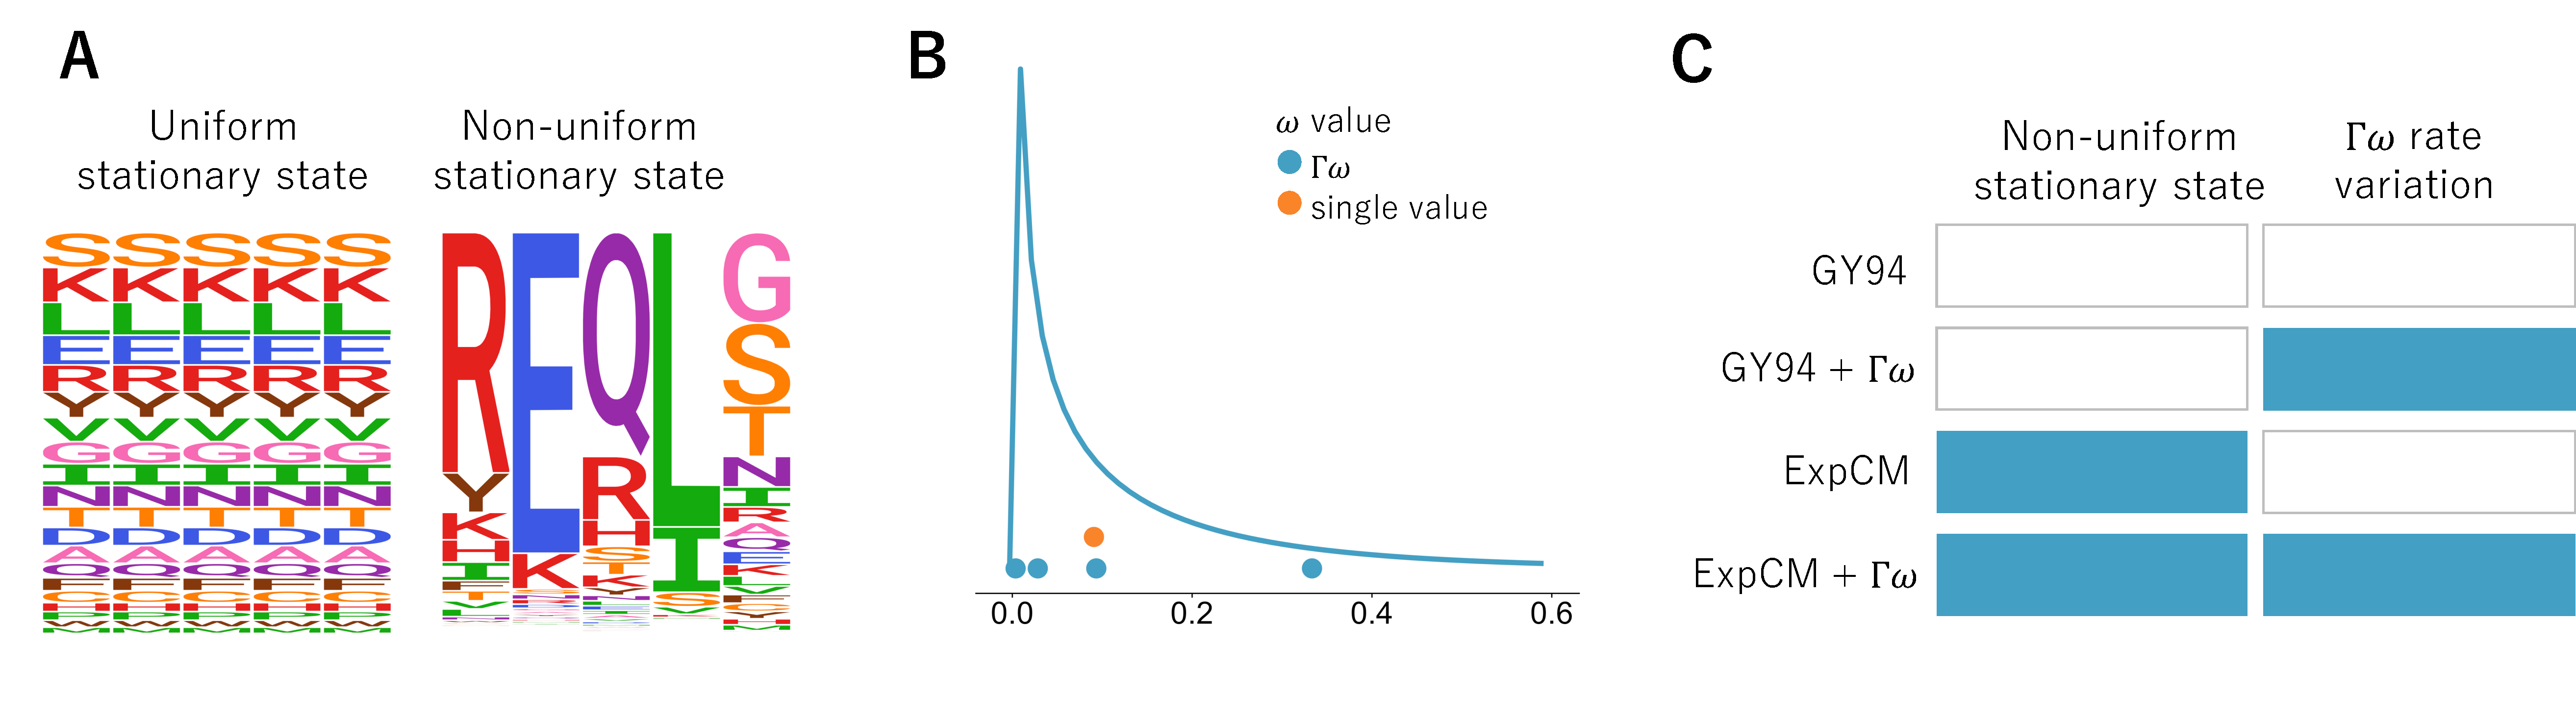
\includegraphics[width=0.90\textwidth]{figures/model_feature.pdf}}
\caption{\label{fig:model_feature}
\textbf{Different ways of modeling site-to-site variation in purifying selection.}
(A) The relative rate of non-synonymous change, $\omega$, can be defined as one, gene-wide average or allowed to vary following some statistical distribution.
In order to achieve computational tractability, the distribution is discretized into $K$ bins and $\omega$ is set to the mean of each bin. 
A $\Gamma$ distribution with $K=4$ bins is shown here. 
(B) Substitution model stationary states can either be identical at every site in the protein or allow to vary from site to site. 
(C) Substitution models can both, one, or neither of these features and we use models from the GY94 and ExpCM families to represent all possible combinations. 
}
\end{figure}

Proteins evolve under both purifying selection to maintain their structure and function. 
This purifying selection is not homogenous across sites in a protein.
It is also not homogenous across the different amino acids at a given site.
For instance, some protein sites strongly prefer hydrophobic amino acids, others may be constrained to just one or a few amino acids, and yet others may tolerate many amino acids.
In general, these constraints are highly idiosyncratic among sites, and so pose a challenge for phylogenetic substitution models.

The most common strategy to model rate variation is to allow the rate of non-synonymous change to vary among sites following some statistical distribution.
For example, in the M5 of \cite{yang2000codon} the implied dN/dS parameter, $\omega$, follows a gamma distribution (GY94+$\Gamma\omega$, \ref{fig:model_feature}A).
Under the GY94+$\Gamma\omega$ and other such models, some sites have a higher rate of non-synonymous change than others. 
However, this rate is agnostic to the amino-acid identities themselves, and so all non-synonymous changes at at given site are treated equally. 

In contrast, so-called ``mutation-selection'' models~\citep{halpern1998evolutionary} account for purifying selection by explicitly defining a different set of amino-acid preferences at each site in the protein. 
This more mechanistic formulation, without an arbitrary statistical distribution, results in a site-specific stationary state (\ref{fig:model_feature}B). 
These models better capture the site-to-site differences in amino-acid composition that is an obvious features of real proteins, and indeed they generally better describe actual evolution than models with only rate variation~\citep{lartillot2004bayesian, le2008phylogenetic, rodrigue2010mutation,hilton2017phydms,bloom2014experimentally}.
The specificity of mutation-selection models comes at a cost in the form of an increased number of parameters. 
While codon substitution models with uniform stationary states typically have $<$20 parameters, mutation-selection models must specify 19 parameters for \emph{each} site (the stationary state is for 20 amino acids whose frequencies are constrained to sum to one).
This corresponds to $19\times L$ parameters for a protein of length $L$, or $\sim 10^4$ parameters for a typical size protein.
As with all parameter-rich models, it is important to obtain values for these parameters using some method that avoids overfitting \skhcomment{cite rodrigue paper}.
Here we will primarily use experimentally informed codon models (ExpCM)~\citep{bloom2014experimentally, hilton2017phydms, bloom2017identification} which define values for these parameters \textit{a priori} from deep mutational scanning experiments~\citep{araya2011,fowler2010high} so they do not need to be fit from phylogenetic data.
Therefore, the number of remaining free parameters that are fit from the phylogenetic data for an ExpCM are similar to a non-site-specific substitution model.
Alternative strategies of obtaining parameters for site-specific stationary states via Bayesian\skhcomment{cite} or maximum-likelihood estimation\skhcomment{cite} are discussed in the last section of the Results.

Finally, these two strategies to account for purifying selection, $\Gamma\omega$ rate variation and site-specific stationary states, are not mutually exclusive. 
Some proteins may be better modeled as a combination of the two. 
Therefore, we will use models from the GY94 (uniform stationary state) and ExpCM (site-specific stationary state) families with and without $\Gamma\omega$ rate variation (\ref{fig:model_feature}C) to examine the effects of each strategy on branch length estimation. 

\subsection*{Effect of stationary state and rate variation on branch length estimation}

\begin{figure}[H]
\centerline{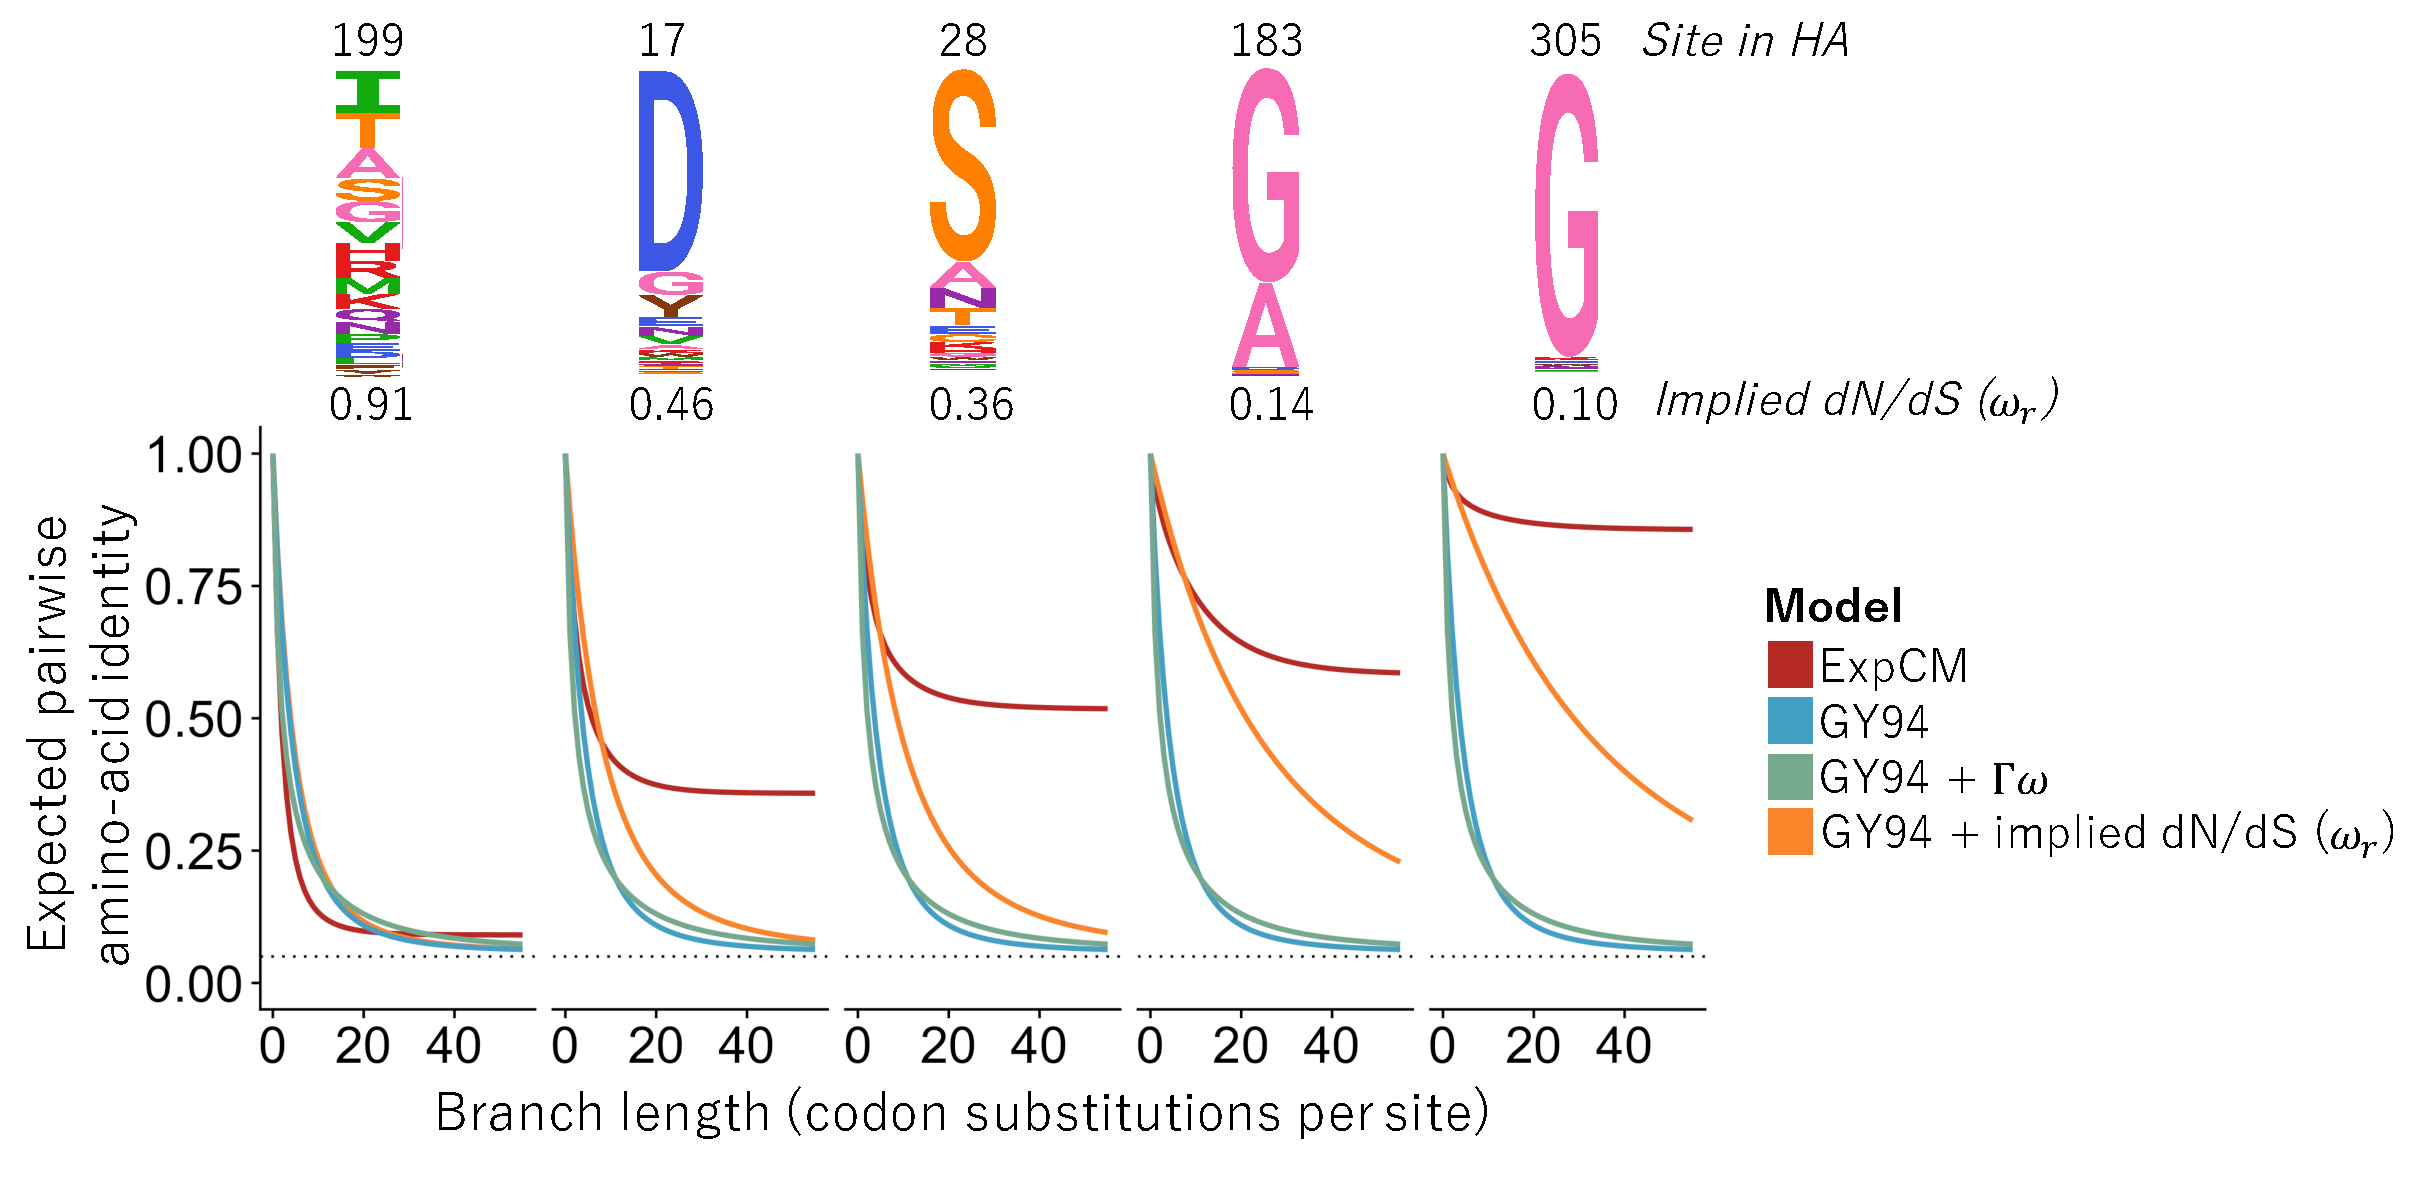
\includegraphics[width=0.90\textwidth]{figures/decay.pdf}}
\caption{\label{fig:decay}
\textbf{Effect of stationary state and rate variation on long branch estimation.}
The expected pairwise amino-acid identity for five sites in influenza hemagglutinin (HA) for four different substitution models calculated using \ref{eq:f}. 
The logoplots show the HA amino-acid preferences from a deep mutational scan performed by \cite{doud2016accurate}. 
The implied dN/dS value was calculated from the ExpCM following \cite{spielman2015relationship} (\ref{eq:w_r}).
\skhcomment{ Maybe change long branch length to expected asymptotic sequence divergence.}
}
\end{figure}

Given a single branch, a substitution model transforms sequence divergence into branch length, which is proportional to time under a molecular clock assumption. 
However, every substitution model has a stationary state, defining the expected sequence composition after a long evolutionary time. 
In \ref{fig:decay}, the stationary state is represented by the long ``tails" where the expected sequence divergence remains constant as time increases. 

By definition, the expected sequence composition varies from site to site for the site-specific stationary state models (\ref{fig:decay} ExpCM, red) but is constant across sites for the uniform stationary state models (\ref{fig:decay} GY94, blue).
The biggest difference in stationary state between the models is at constrained sites, such as site 305 in \ref{fig:decay}. 
At such a site, the ExpCM would estimate a much longer branch than the GY94 given the observed divergence of a set of sequences. 

Rate variation, as modeled by $\Gamma\omega$, affect the rate at which stationary state is approached by not the sequence composition at stationary state itself. 
Stationary state is a fundamental feature of stochastic matrices and is invariant to multiplicative terms, such as $\omega$. 
In \ref{fig:decay}, GY94+$\Gamma\omega$ (green) takes longer to reach the stationary state than GY94 (blue) but stationary state for each model is identical. 

This means even complex modeling of the $\omega$ to account for purifying selection will not affect the expectation at evolutionary equilibrium. 
We inferred a site-specific $\omega$ value from the ExpCM \citep{spielman2015relationship} and applied these values to the GY94 model, GY94+$\Gamma\omega$ (\ref{fig:decay} yellow). 
At constrained sites, this model takes even longer to reach stationary state than the GY94+$\Gamma\omega$ but the eventual stationary state is identical to both the GY94 and GY94+$\Gamma\omega$ stationary state. 

No matter how ``well" a model accounts for site-to-site rate variation, it will underestimate long branches with a uniform stationary state. 

\subsection*{Failure to account for site-specificity leads to branch length underestimation.}

\begin{figure}[H]
\centerline{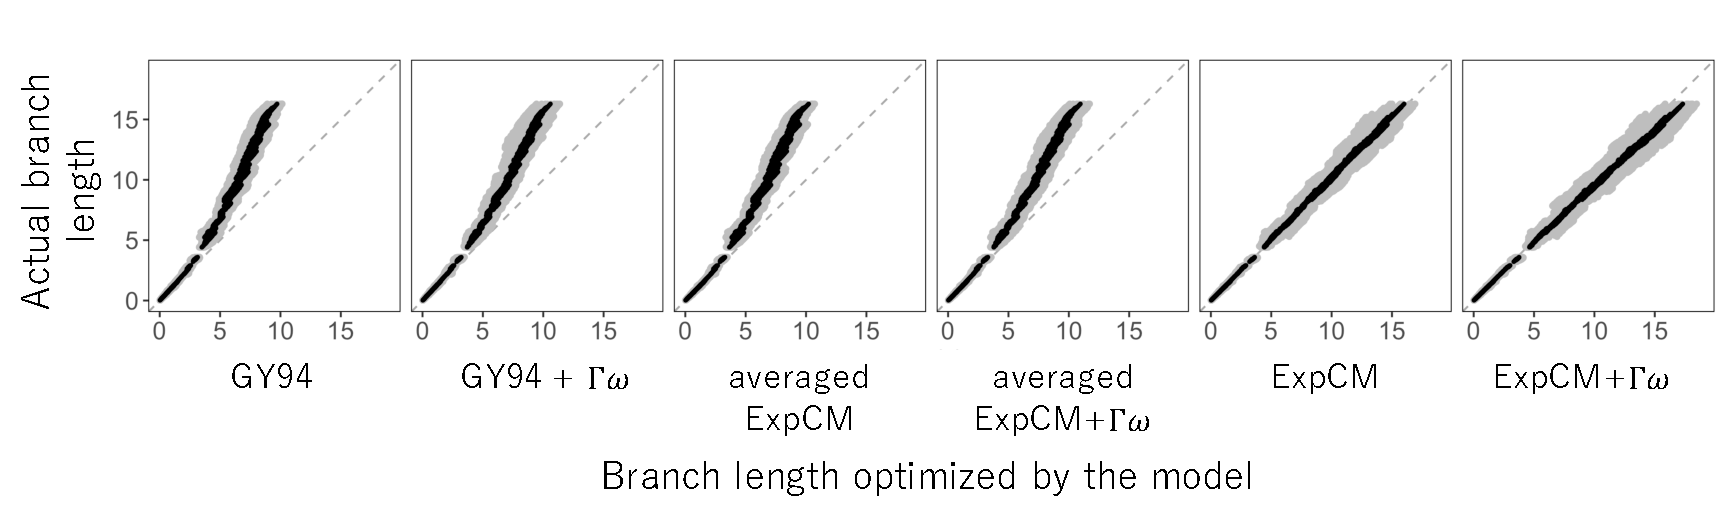
\includegraphics[width=0.85\textwidth]{figures/simulations}}
\caption{\label{simulations}
\textbf{Model performance under simulated, site-specific data.} 
Alignments were simulated under an ExpCM along an HA tree and the branches were re-optimized by a model from the ExpCM or YNGKP family. 
The averaged ExpCMs amino-acid frequencies defined by the average preference of that amino acid across all sites in the protein. 
While these models extract information from the deep mutational scanning experiment, they are not site-specific. 
Grey points represent the length of one branch and the black points are the mean branch lengths over ten simulations. 
The grey, dashed line is the reference line $y=x$, depicting the behavior of a model which is an unbiased estimator of the simulated branch length. 
}
\end{figure}

Next, we wanted to test the effect of substitution model stationary state on branch length estimation given sequences with site-specific amino-acid frequencies. 
We simulated sequences under an ExpCM and re-inferred the branch lengths using different substitution models described in \ref{fig:model_feature}C.

The ExpCM and the ExpCM+$\Gamma\omega$ estimated the branch lengths of the simulated sequences accurately. 
This accuracy is expected as this was the model the sequences were simulated under. 
The variance in the estimation of a given branch increases between the simulations increased as branch length increased. 
However, this error is not biased towards over- or underestimation. 

The models with a uniform stationary state consistently underestimate the long branches. 
This underestimation is seen with both the GY94 and the GY94+$\Gamma\omega$, indicating that accounting for rate variation via the rate parameter cannot prevent branch length underestimation at these long branches. 
The ExpCM can also be transformed into a uniform stationary state model by setting the amino-acid at every site to the average value for that amino acid across all sites. 
In contrast to the GY94 models, this average control does not have preference for amino acid and does extract some information from the experiments, but like the GY94 models the stationary state is uniform across sites. 
These models performed similarly to the GY94 and GY94+$\Gamma\omega$ and underestimated long branches. 

These simulations show that when the sequences have site-specific amino-acid frequencies, models with uniform stationary states cannot accurately estimate branch lengths and, will in fact, underestimate long branches. 	

\subsection*{empirical Data}

\begin{figure}[H]
\centerline{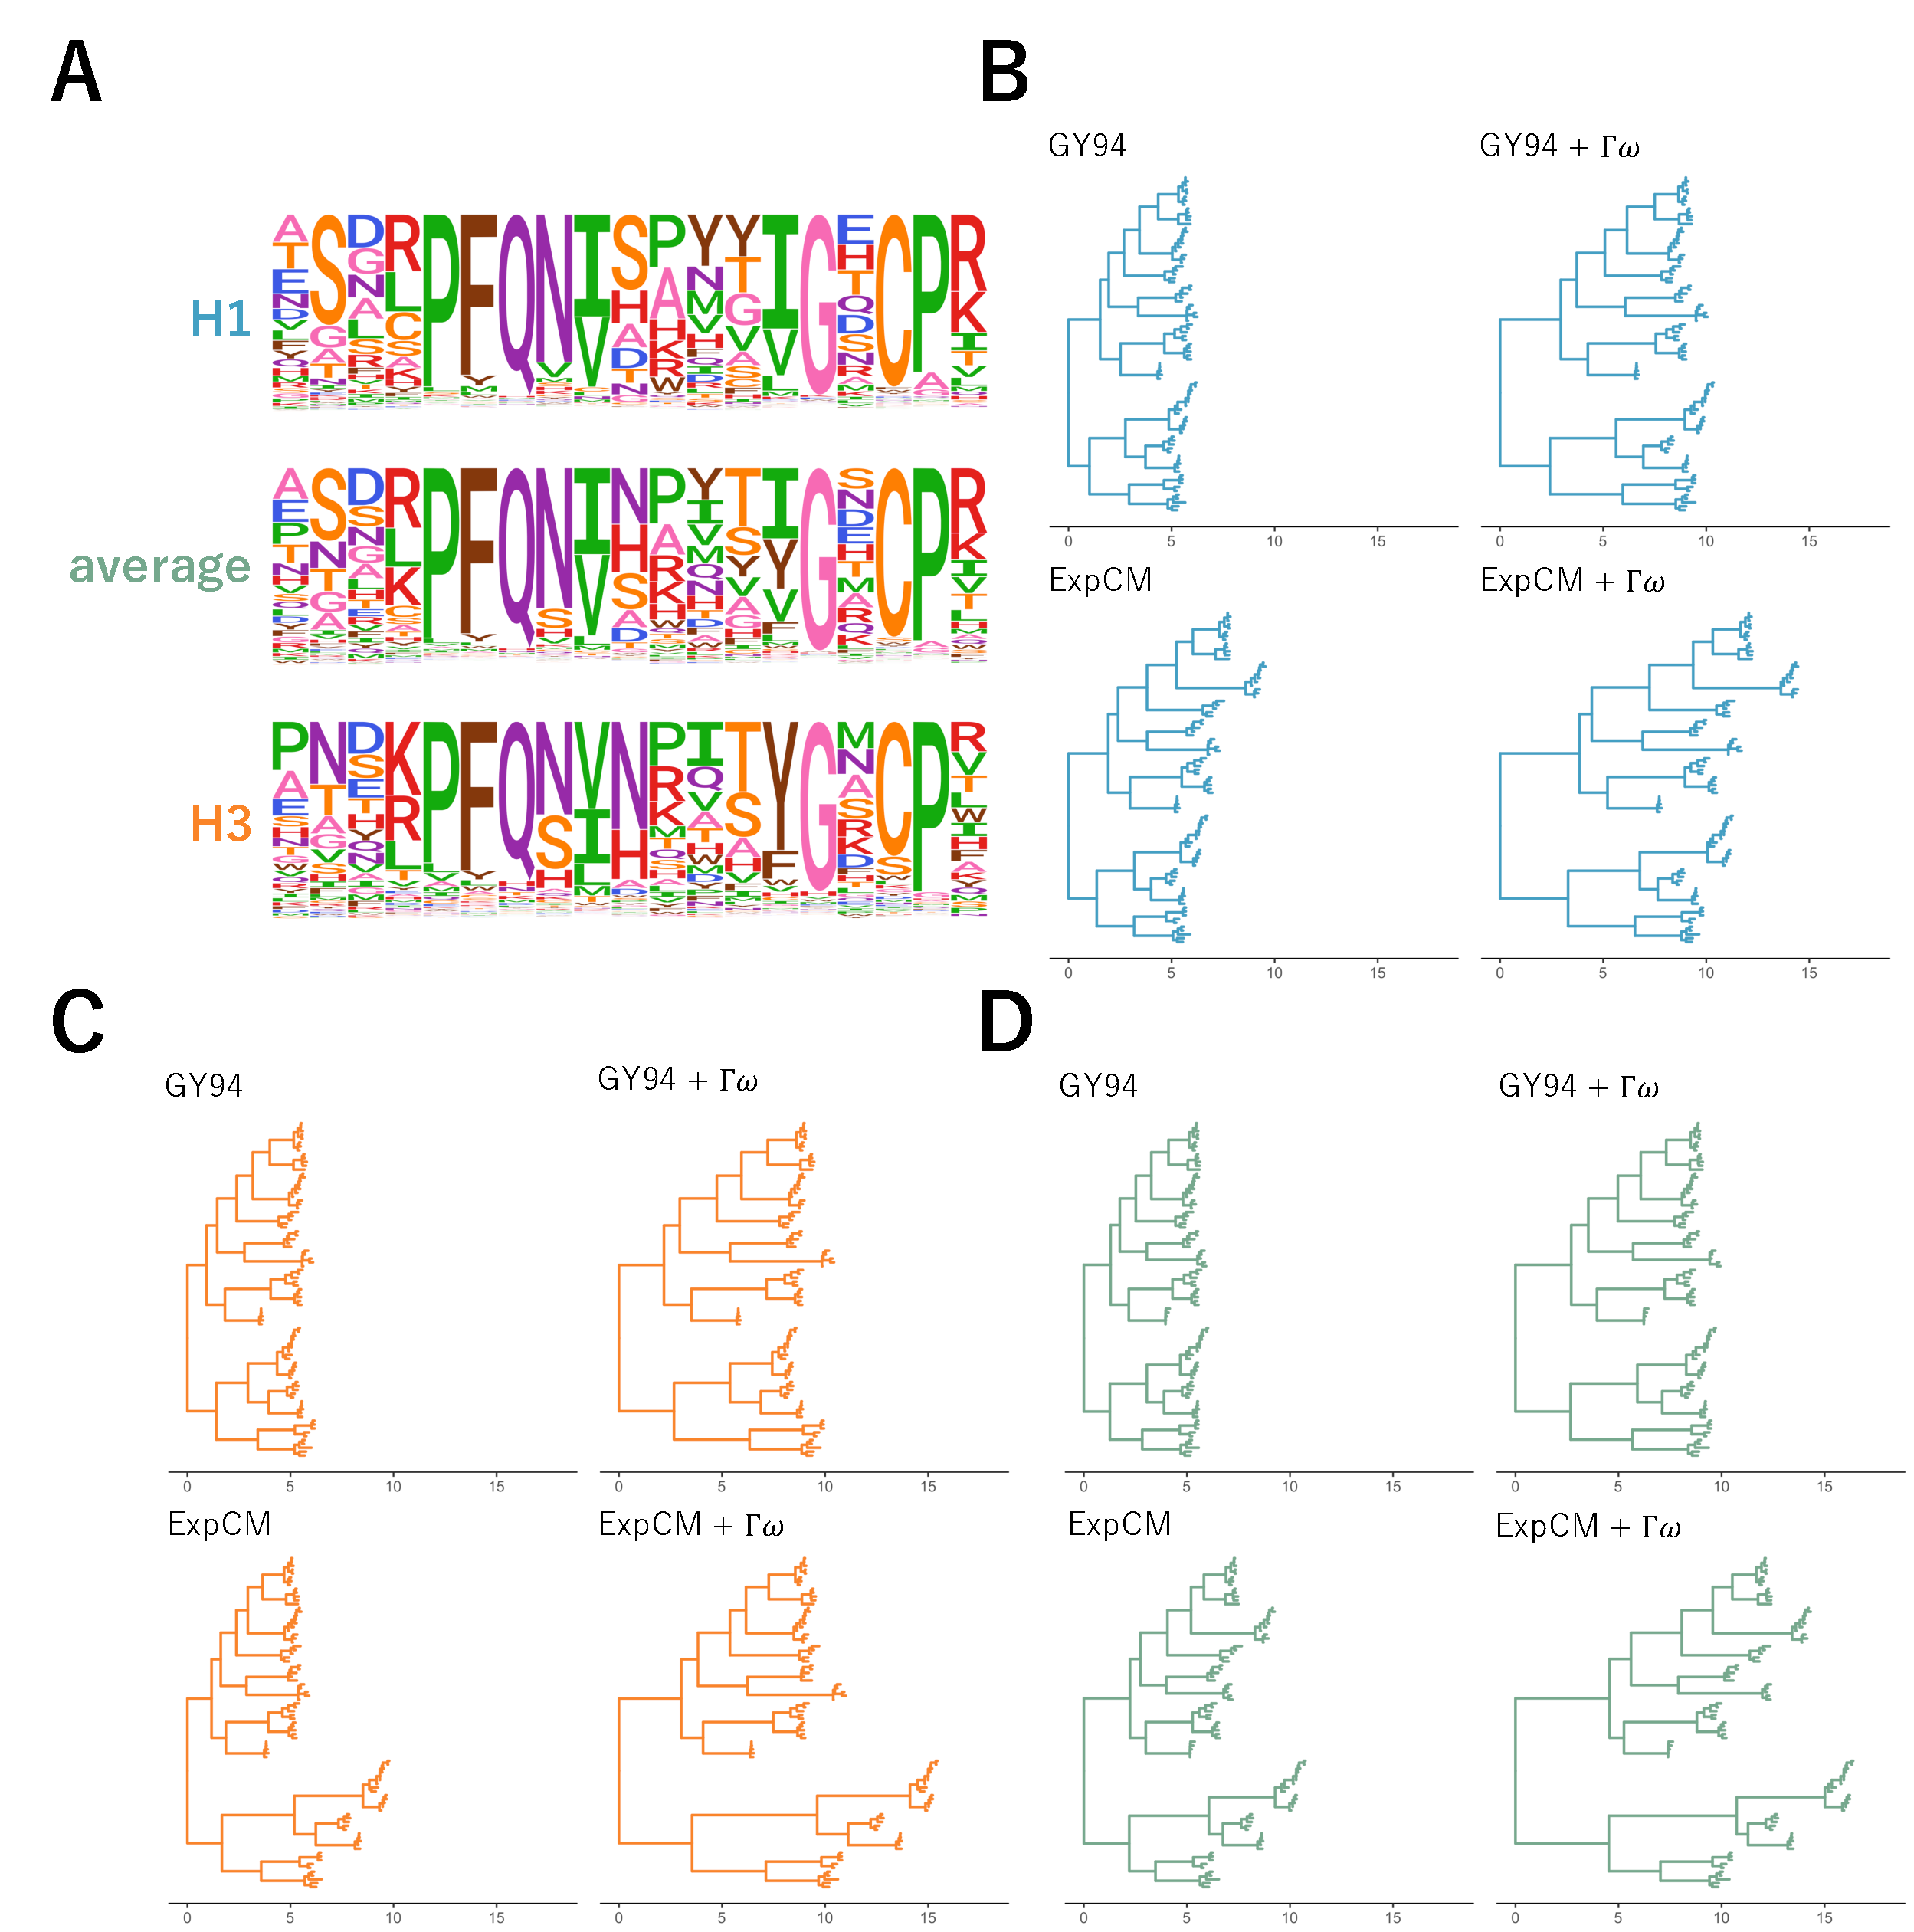
\includegraphics[width=0.8\textwidth]{figures/empirical_trees.pdf}}
\caption{\label{fig:empirical_trees}
\textbf{Trees optimized with an ExpCM defined by H1 preferences lengthen branches from the focal H1 sequence compared to GY94 models.} ).
}
\end{figure}

\begin{table}[t!]
\caption{\label{tab:empirical_data}
Model comparison for Fig.~\ref{fig:empirical_trees}.\skhcomment{GY94+$\Gamma\omega$ has one $\omega$ of 0 because of rounding.}} 
     \begin{tabular}{cccccccccc}
        \hline
         Model & {\shortstack{Stationary\\ State}} & $\Gamma\omega$ & $\Delta$AIC & {\shortstack{Log\\ Likelihood}} & {\shortstack{$\omega$\\ (implied dN/dS)}} & {\shortstack{stringency\\ parameter}}\\ \hline
       	ExpCM + $\Gamma\omega$ (H1+H3 avg) & yes & yes & 0 & -487510 & 0.19,  0.50,  0.90,  1.86 &  1.70, \\
	ExpCM (H1+H3 avg) & yes & no &  950 & -492270 & 0.15 & 1.78\\
	ExpCM + $\Gamma\omega$ (H1) & yes & yes & 13060 & -494040  & 0.13 ,  0.44,  0.91,  2.16 & 1.12\\
	ExpCM + $\Gamma\omega$ (H3) & yes & yes & 17370 & -49620 & 0.09,  0.33,  0.72,  1.77 & 1.28\\
	ExpCM (H1) & yes & no & 2556 & -50030 &  0.13 & 1.22\\
	ExpCM (H3) & yes & no &  3197 & -50350 & 0.12 & 1.45\\
	GY94 + $\Gamma\omega$ & no & yes & 4719 & -51106 & 0.00,  0.03,  0.08,  0.26 & N/A \\
	GY94 & no & no & 7625 & -52560  & 0.07 & N/A\\
      \end{tabular}
\end{table}

Next, we tested the effect of substitution model on branch length estimation using influenza HA sequences. 
Like the simulated sequences, we assume the influenza HA sequences have site-specific frequencies but unlike the simulations we do not know the underlying model. 

Influenza HA proteins are group into two groups, based on phylogenetic and antigenic properties. 
Each HA subtype within the larger groups contains closely related sequences and is connected to the other HA subtype by long branches. 
The most diverged homologs on this tree are upwards of 60\% diverged on the amino acid level. 
Consequently, the HA tree is a good model to look at long branch estimation as the there are numerous long branches spread more or less ``evenly" across the entire tree. 

We built an HA tree sequences from 14 of the 18 subtype groups, excluding subtype groups with very few sequences. 
Then we optimized the branch lengths on the tree using models from the GY94 and ExpCM families. 
We compared ExpCMs defined by two different deep mutational scans measured in two different genetic background. 
One deep mutational scan was measured in an H1 background and the other was measured in an H3 background. 
The two focal sequences of these deep mutational scan are only 42\% identical. 
Comparison of these two models allowed us to examine the effect of ExpCM focal sequence on the branch length estimation. 
Additionally, because the models we used represent all possible combinations of $\Gamma\omega$ rate variation and site-specific stationary state, we were able to examine the effect of each of these features while controlling for the presence of the other. 

The addition of $\Gamma\omega$ rate variation or site-specific stationary state increased the branch lengths estimated. 
The addition of site-specific stationary state and $\Gamma\omega$ rate variation each increased branch length compared to the model without the feature. 
The longest branches were estimated with the ExpCM+$\Gamma\omega$, which included both features. 

However, the branch length extension for the ExpCM was not uniform across the entire tree. 
The longest branch length extension is on branches near the focal sequence of the deep mutational scan. 
The greatest difference between the GY94 and the ExpCM (H1 preferences) is on branches near the H1 clade (black circle) while the greatest difference between the GY94 and the ExpCM (H3 preferences) is on the branches near the H3 clade (black triangle). 
This indicates that the stationary state described by the DMS preferences is much more accurate near the focal sequence of the scan. 

This result is not entirely surprising. 
DMS measures the effect of single amino-acid changes in the context of a single genetic background. 
However, it is expected that there would be epistatic changes and interactions with such highly diverged homologs. 
That is, the effect of an amino acid change at one site in the protein might be affected by the amino acid identity at another site in the protein. 
This would cause the preferences, and consequently the stationary state, to ``shift" across the tree and would explain why there is some locality to our ExpCMs. 
To test the effect of ``sampling" multiple preference sets, inferred the branch lengths using an ExpCM defined by the average of the H1 and H3 preferences. 
This model estimated longer branches from both the H1 and H3 clades compared to the GY94 model, indicating that there are these shifts across the entire tree. 

\subsection*{Competing effects of shifting preferences and long branches.}

\begin{figure}[H]
\centerline{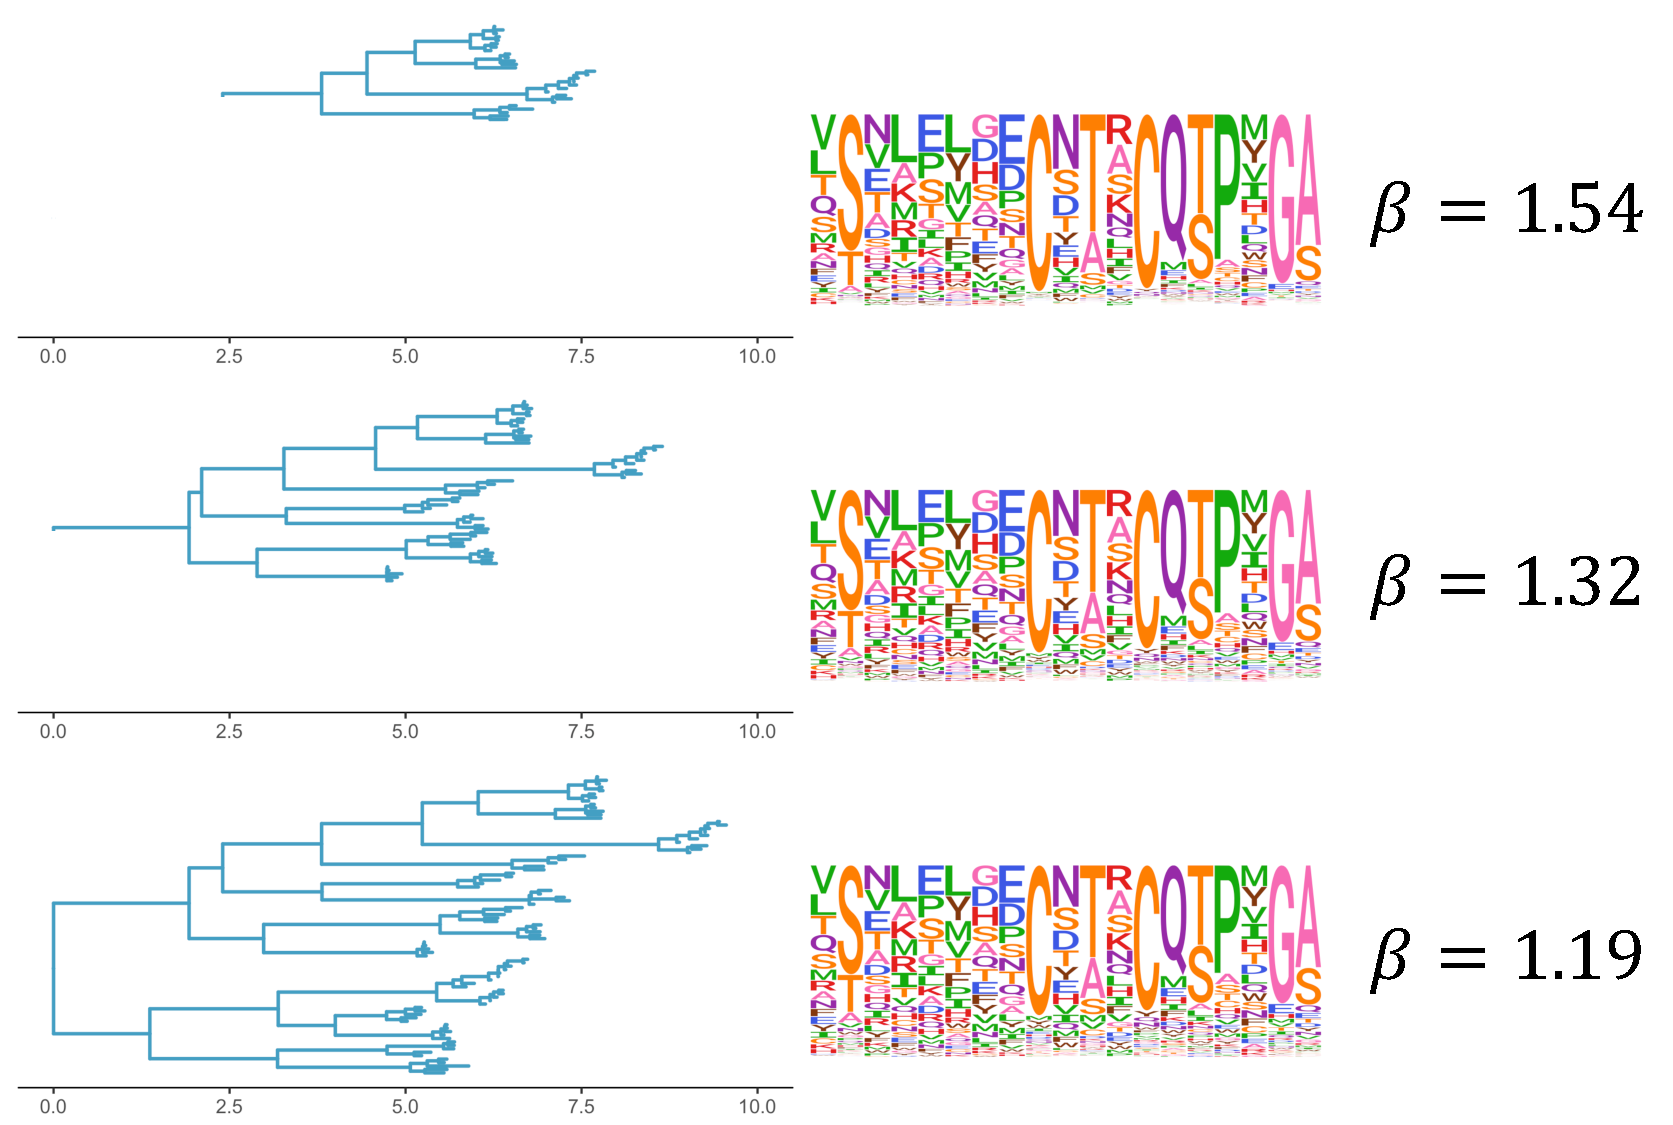
\includegraphics[width=0.85\textwidth]{figures/doud_compete_2}}
\caption{\label{fig:doud_compete}
\textbf{The ExpCM defined by H1 preferences lengthen longer branches on the HA tree.} 
\textbf{(A)} An HA alignment was subsampled to create three smaller alignments with varying degrees of divergence from the focal H3 sequence, referred to as "low", "intermediate", and "high". 
\textbf{(B)} The phylogenetic tree of the "high" alignment. 
The colors denote the alignment and the black circle denotes the focal H3 sequence. 
\textbf{(C)} The value of the ExpCM and ExpCM+$\Gamma\omega$ stringency parameter $\beta$ decreases as the divergence from the focal H3 sequence increases. 
\textbf{(D)} Comparisons of branch lengths optimized by the four substitution models for the varying degrees of divergence. 
Black points represent branches from the focal H3 sequence and grey points represent all other branches.  
The branch lengths are in average number of codon substitutions per site. 
}
\end{figure}

We further investigated the effect of ``shifting" preferences by comparing behavior of ExpCM across trees with increasing overall divergence from the focal sequence of the deep mutational scans. 
Based on our results with the large HA trees, we expected the preferences to be more "relevant" on trees which have a low overall sequence divergence from the DMS focal sequence. 

We use the value of the ExpCM stringency parameter to measure the ``relevance" of a given DMS preference set and tree. 
A stringency parameter with a value greater than one indicates that selection in nature prefers the same amino acids as selection in lab but with greater strength, or that the preferences are ``relevant" to evolution in nature. 
Conversely, when the stringency parameter is fit to a value close to zero, the preferences are not ``relevant" and de-emphasize the measurements from the lab so that the preferences are flat. 
Using the ExpCM (H1 preferences), we observe an inverse relationship between overall divergence and the stringency. 
As the tree includes more and more sequences which are further from the focal sequence, the relevance of the preferences declines. 
This indicates that the preferences truly are most relevant on trees with sequences closely related to the focal sequence (short branches). 

While the preferences are most relevant for the trees with short branches, due to the low divergence from the focal sequence, the effect of site-specific stationary states on branch length estimation is most important on long branches. 
On the low divergence tree, with the most ``relevant" preferences, roughly the same branch length estimated by the GY94+$\Gamma\omega$  and the ExpCM+$\Gamma\omega$. 
In fact, it is not until the high divergence tree that a true effect is seen, in the branches from the focal sequences. 
The effect from site-specific substitution models doesn't really have an effect until the branch lengths are a particular length. 

This leads to a regime with competing effects. 
As the branch lengths increase, the ``importance" of having a site-specific stationary state increases. 
At the same time, the ``relevance" of an given site-specific stationary decreases as the divergence increases. 
Current models which have one stationary state across the entire tree, site-specific or not, will not be able to address this tension. 

\subsection*{\texttt{phylobayes}}

Finally, we compared the branch lengths estimated by ExpCM to branch lengths estimated by another site-specific stationary state model. 
We inferred the branch lengths on the ``high" divergence tree using the mutation-selection model implement in \texttt{phylobayes}. 
Unlike the ExpCM, this mutation-selection model in \texttt{phylobayes} 

\begin{figure}[H]
\centerline{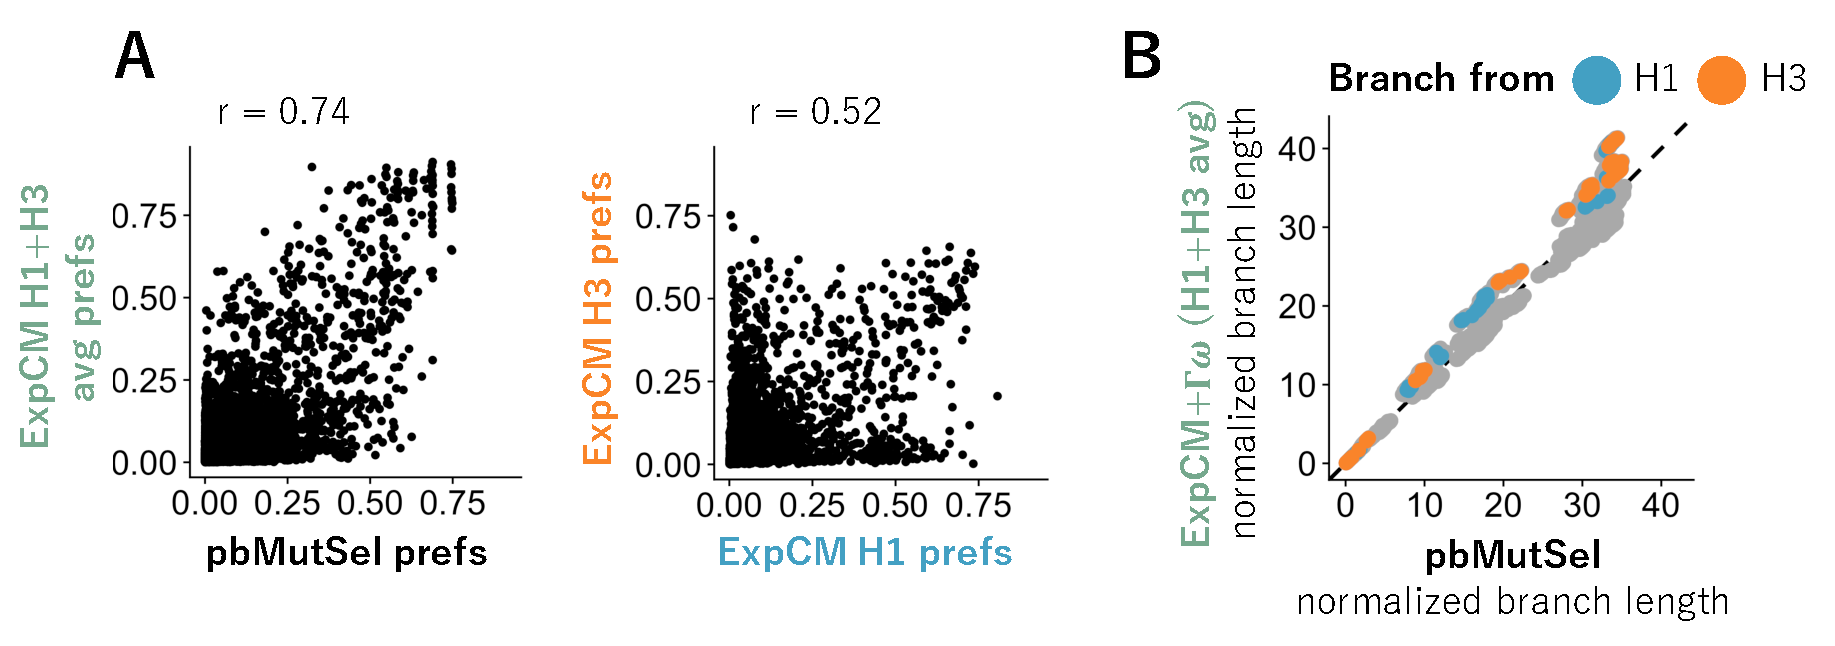
\includegraphics[width=0.5\textwidth]{figures/phylobayes.pdf}}
\caption{\label{fig:phylobayes}
\textbf{Comparison of ExpCM and phylobayes}
\skhcomment{y=x line too faint?}
}
\end{figure}

\section*{Conclusion}

\begin{enumerate}
  \item We don't allow any of the models to vary by lineage. 
\end{enumerate}

\newpage
\section*{Materials and Methods}

\subsection*{Substitution models}
\subsubsection*{GY94 models}
\subsubsection*{ExpCMs}
We recap the \textbf{Exp}erimentally Informed \textbf{C}odon \textbf{M}odel (ExpCM) \citep{bloom2014experimentally,bloom2014informed,bloom2017identification,hilton2017phydms} to introduce nomenclature. 

In an ExpCM, rate of substitution $P_{r,xy}$ of site $r$ from codon $x$ to $y$ is written in mutation-selection form~\citep{halpern1998evolutionary,mccandlish2014modeling,spielman2015relationship} as
\begin{equation}
P_{r,xy} = Q_{xy} \times F_{r,xy}
\end{equation}
where $Q_{xy}$ is proportional to the rate of mutation from $x$ to $y$, and $F_{r,xy}$ is proportional to the probability that this mutation fixes.
The rate of mutation $Q_{xy}$ is assumed to be uniform across sites, and takes an HKY85-like~\citep{hasegawa1985dating} form:
\begin{equation}
Q_{xy} = 
\begin{cases}
\phi_w & \mbox{if $x$ and $y$ differ by a transversion to nucleotide $w$} \\
\kappa \phi_w & \mbox{if $x$ and $y$ differ by a transition to nucleotide $w$} \\
0 & \mbox{if $x$ and $y$ differ by $>1$ nucleotide.}
\end{cases}
\end{equation}
The $\kappa$ parameter represents the transition-transversion ratio, and the $\phi_w$ values give the expected frequency of nucleotide $w$ in the absence of selection on amino-acid substitutions, and are constrained by $1 = \sum_w \phi_w$.

The deep mutational scanning data are incorporated into the ExpCM via the $F_{r,xy}$ terms.
The experiments measure the preference $\pi_{r,a}$ of every site $r$ for every amino-acid $a$.
The $F_{r,xy}$ terms are defined in terms of these experimentally measured amino-acid preferences as
\begin{equation}
\label{eq:Frxy}
F_{r,xy} = 
\begin{cases}
   1 & \mbox{if $\mathcal{A}\left(x\right) = \mathcal{A}\left(y\right)$} \\
   \omega \times \frac{\ln\left[\left(\pi_{r,\mathcal{A}\left(y\right)} / \pi_{r,\mathcal{A}\left(x\right)}\right)^{\beta}\right]}{1 - \left(\pi_{r,\mathcal{A}\left(x\right)} / \pi_{r,\mathcal{A}\left(y\right)}\right)^{\beta}} & \mbox{if $\mathcal{A}\left(x\right) \ne \mathcal{A}\left(y\right)$}
   \end{cases}
\end{equation}
where $\mathcal{A}\left(x\right)$ is the amino-acid encoded by codon $x$, $\beta$ is the stringency parameter, and $\omega$ is the relative rate of nonsynonymous to synonymous substitutions after accounting for the amino-acid preferences.
The ExpCM has six free parameters (three $\phi_w$ values, $\kappa$, $\beta$, and $\omega$).
The preferences $\pi_{r,a}$ are \emph{not} free parameters since they are determined by an experiment independent of the sequence alignment being analyzed.

The ExpCM stationary state frequency $p_{r,x}$ of codon $x$ at site $r$ is~\citep{bloom2017identification} 
\begin{equation}
\label{eq:p_rx}
p_{r,x} = \frac{\left(\pi_{r,\mathcal{A}\left(x\right)}\right)^{\beta} \phi_{x_0} \phi_{x_1} \phi_{x_2}}{\sum_z \left(\pi_{r,\mathcal{A}\left(z\right)}\right)^{\beta} \phi_{z_0} \phi_{z_1} \phi_{z_2}},
\end{equation}
\subsection*{Theoretical effect of model choice on branch length}
\subsection*{Effect of model choice on natural sequences}

\subsubsection*{ExpCM + $\Gamma\omega$ and YNGKP M5}


\subsubsection*{Spielman $\omega_{r}$ values inferred from the ExpCM} 
We inferred the average nonsynonymous fixation rate from the ExpCM following~\citet{spielman2015relationship} as 
\begin{equation}
\label{eq:w_r}
\omega_{r} = \frac{\sum_{x} \sum_{y \in N_x} {p_{r,x} \times P_{r,xy}}}{\sum_{x} \sum_{y \in N_x} {p_{r,x} \times Q_{xy}}}
\end{equation}
where $p_{r,x}$ is the stationary state of the ExpCM at site $r$ and codon $x$, $P_{r,xy}$ is the substitution rate from codon $x$ to codon $y$ at site $r$, $Q_{xy}$ is the mutation rate from codon $x$ to codon $y$, and $N_x$ is the set of codons that are nonsynonymous to codon $x$ and differ from codon $x$ by only one nucleotide. 

\subsubsection*{Expected pairwise amino-acid identity}
\textit{Do I need to talk about the branchScale scaling I used?}
The expected pairwise amino-acid identity at a site $r$ over time $t$ for a given model is 
\begin{equation}
\label{eq:f}
\sum_a \sum_{x \in a} p_{r,x} \sum_{y \in a} [M_{r}\left(t\right)]_{xy}
\end{equation}
where $a$ is all amino acids, $p_{r,x}$ is the stationary state of the model at site $r$ and codon $x$, and $[M_{r}\left(t\right)]_{xy}$ is the transition rate from codon $x$ to codon $y$ at site $r$ given time $t$. 

\newpage
\section*{Supplemental Information}

\subsection*{Model Parameters for the simulations}

\begin{suppfig}[H]
\centerline{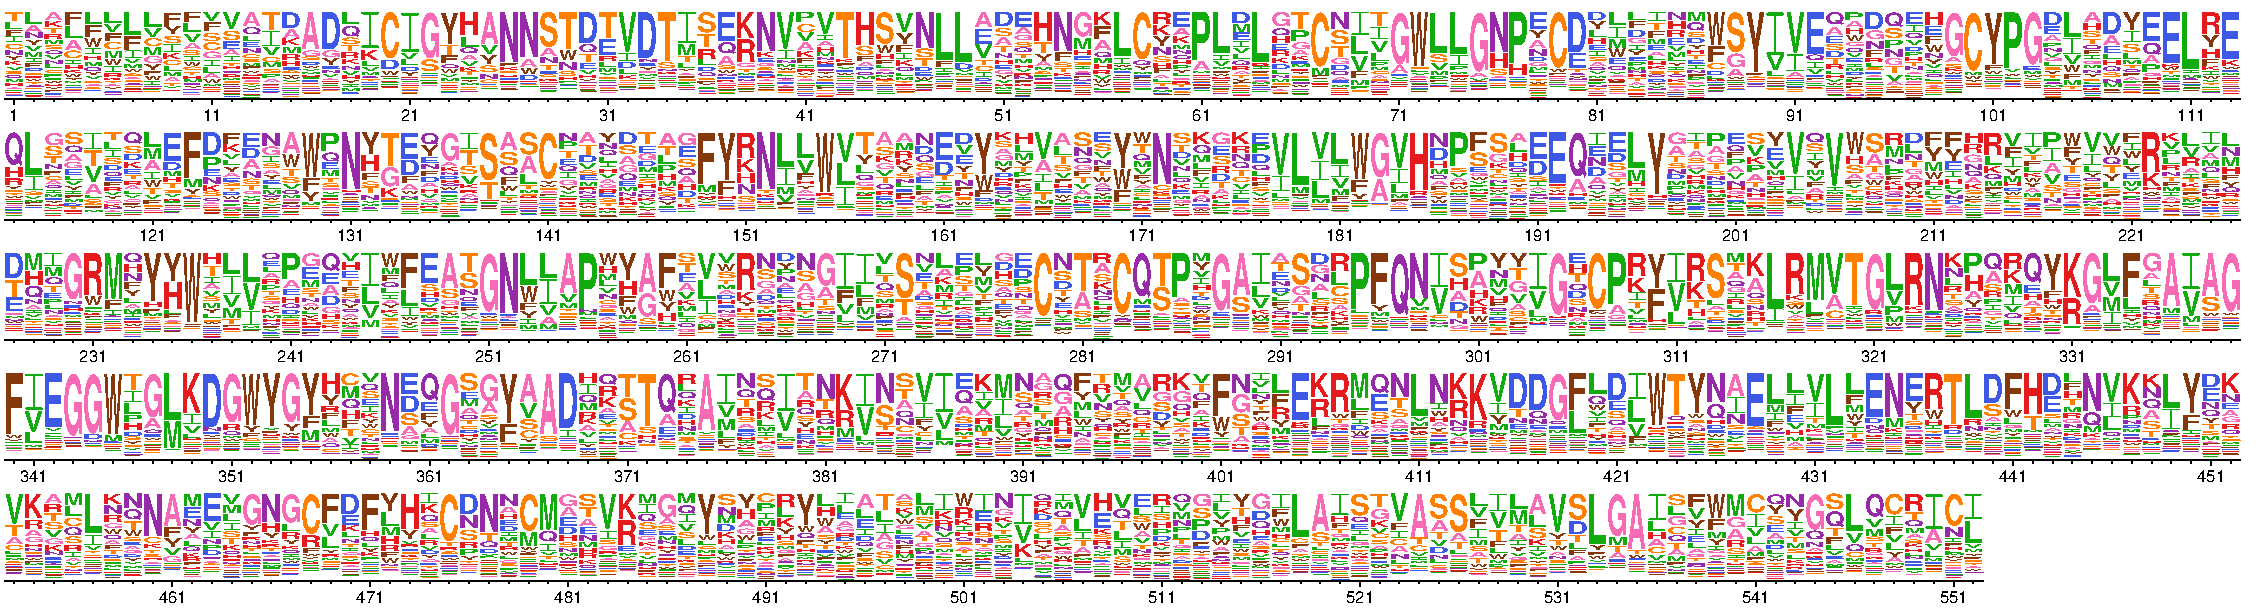
\includegraphics[width=\textwidth]{figures/prefs_doud}}
\caption{\label{suppfig:prefs_doud}
\textbf{H1 preferences measured by \cite{doud2016accurate} rescaled with the ExpCM stringency parameter optimized in \ref{fig:tree_doud}A  ($\beta = 1.19$)} 
\skhcomment{I need to change the $\beta$ value when the new \texttt{phydms} results finish running.}
}
\end{suppfig}

\begin{suppfig}[H]
\centerline{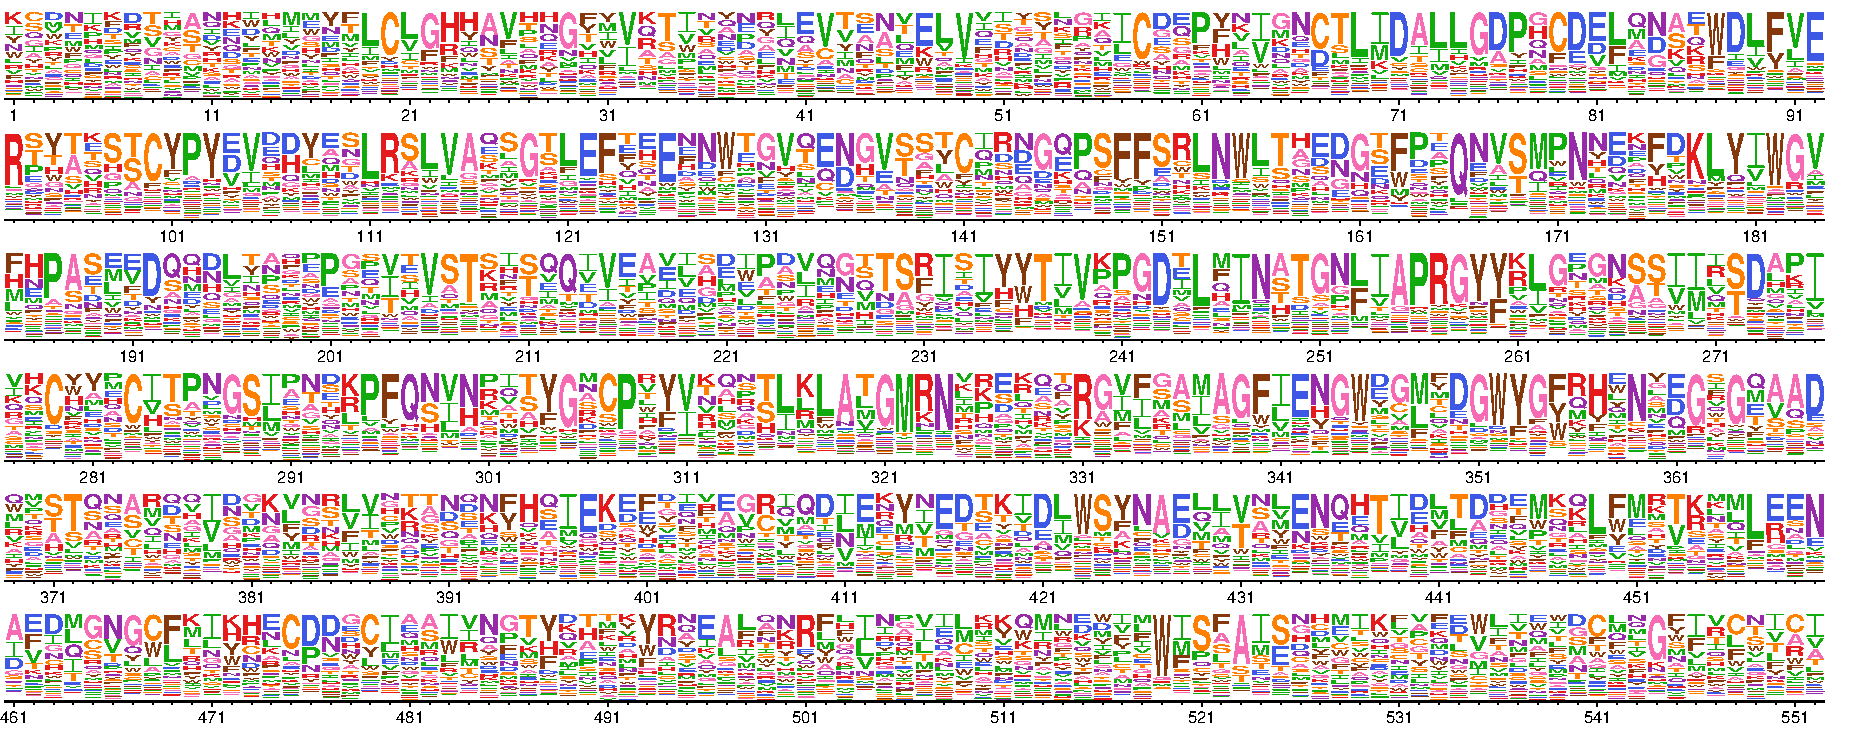
\includegraphics[width=\textwidth]{figures/prefs_lee}}
\caption{\label{suppfig:prefs_lee}
\textbf{H3 preferences measured by \textit{lee} rescaled with the ExpCM stringency parameter optimized in \ref{fig:tree_lee}A  ($\beta = 1.46$)}
\skhcomment{I need to change the $\beta$ value when the new \texttt{phydms} results finish running.} 
}
\end{suppfig}

\begin{suppfig}[H]
\centerline{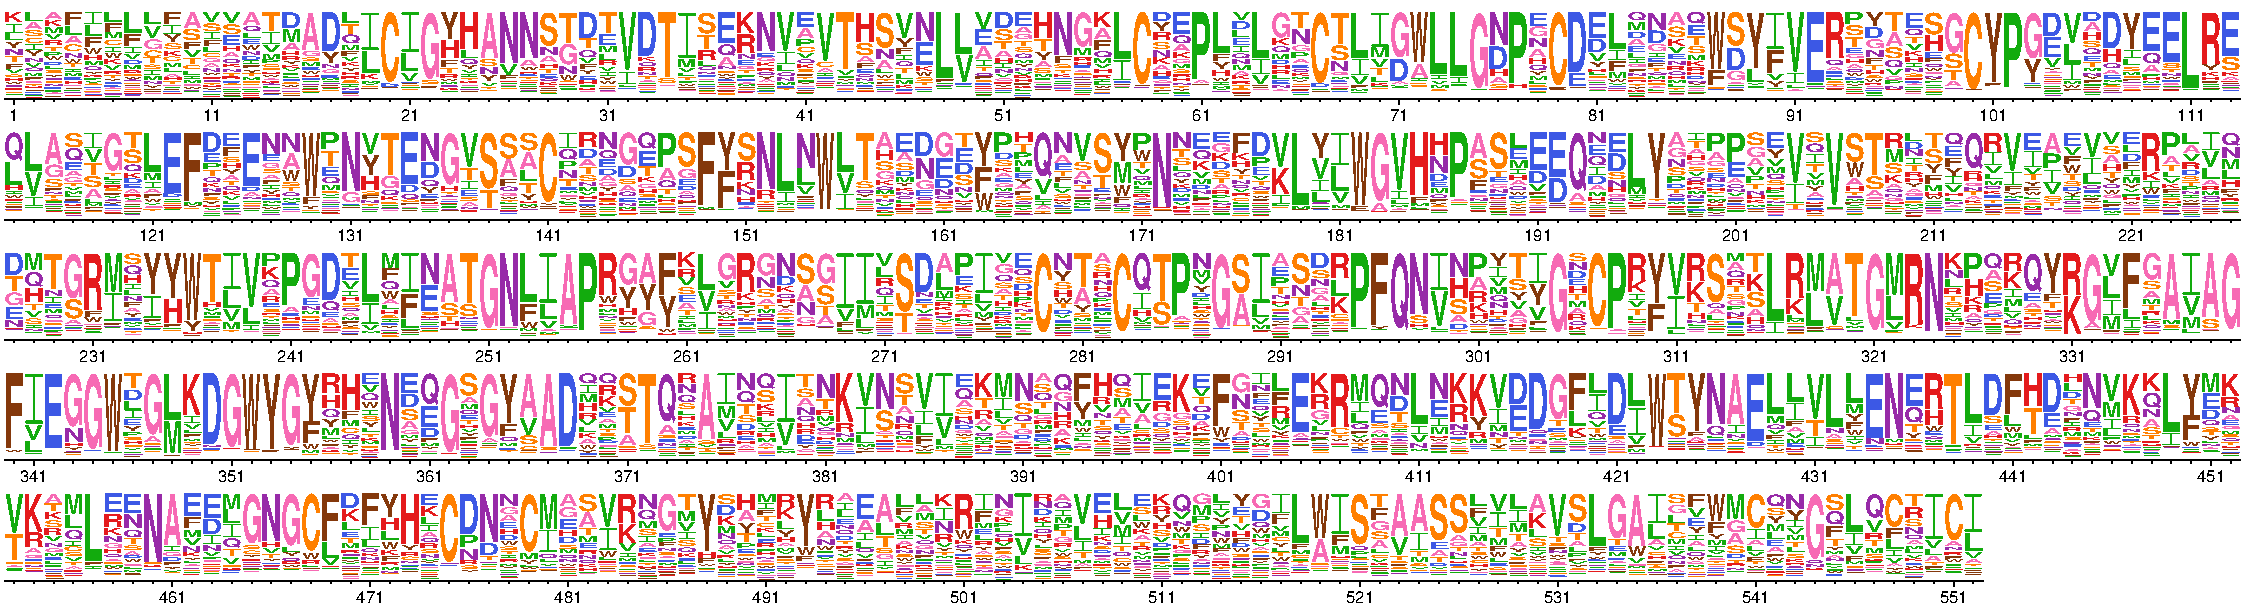
\includegraphics[width=\textwidth]{figures/prefs_average}}
\caption{\label{fig:prefs_average}
\textbf{The average of the H1 preferences measured by \cite{doud2016accurate} and the H3 preferences measured by \textit{Lee} rescaled with the ExpCM stringency parameter optimized in \ref{fig:tree_average}A  ($\beta = 1.77$)}}
\skhcomment{I need to change the $\beta$ value when the new \texttt{phydms} results finish running.}
\end{suppfig}
 


\begin{table}[t!]
\caption{\label{tab:simulation_params}
ExpCM parameters used to simulate sequences in Fig.~\ref{fig:simulation}.}
      \begin{tabular}{ccccc}
        \hline
          Parameter & Value\\ \hline
       	$\beta$ & $1.54$\\
	$\kappa$ & $3.60$\\
	$\omega$ & $0.20$\\
	$\phi_A$, $\phi_C$, $\phi_G$& $0.38$, $0.17$, $0.23$\\
      \end{tabular}
\end{table}

\begin{table}[t!]
\caption{\label{tab:wsn_low_params}
Model parameters used in  Fig.~\ref{fig:decay}.}
      \begin{tabular}{ccccc}
        \hline
          Model & Parameters\\ \hline
          ExpCM & $\beta=1.54196$\\
           & $\kappa=3.47184$\\
           & $\omega=0.219225$\\ 
          YNGKP M0 & $\kappa=2.9984$\\
          & $\omega=0.09076$\\
          YNGKP M5 & $\kappa=2.9984$\\
          & $\omega=0.09076$\\
      \end{tabular}
\end{table}

\begin{suppfig}[H]
\centerline{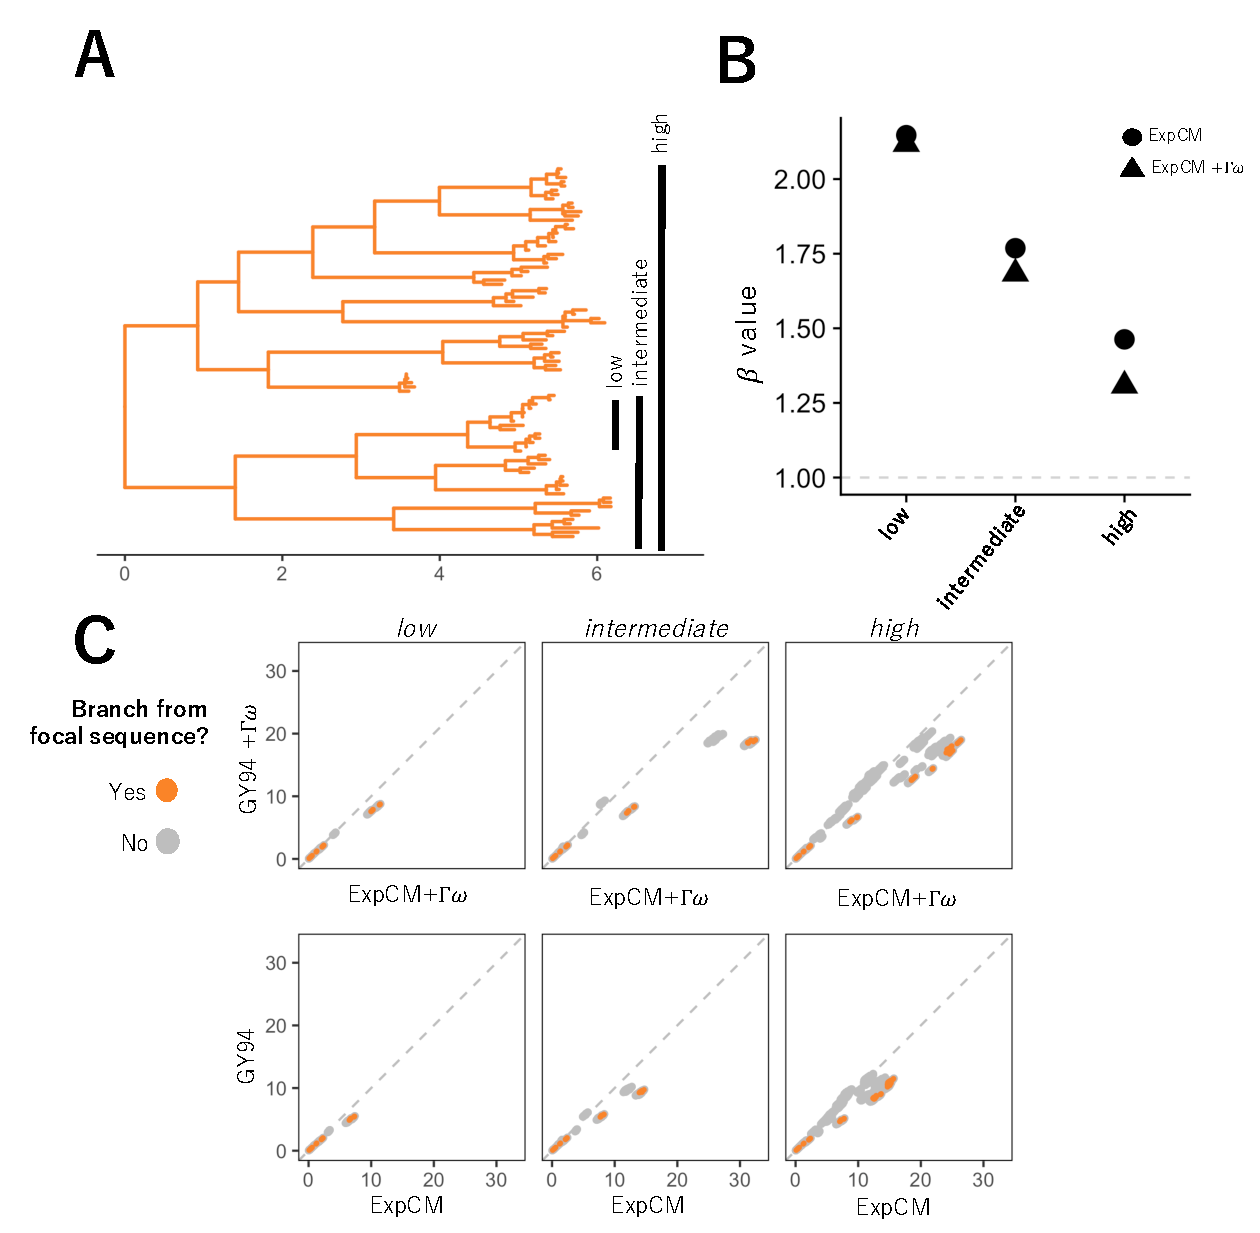
\includegraphics[width=0.85\textwidth]{figures/lee_compete}}
\caption{\label{fig:lee_compete}
\textbf{The ExpCM defined by H1 preferences lengthen longer branches on the HA tree.} 
\textbf{(A)} An HA alignment was subsampled to create three smaller alignments with varying degrees of divergence from the focal H3 sequence, referred to as "low", "intermediate", and "high". 
\textbf{(B)} The phylogenetic tree of the "high" alignment. 
The colors denote the alignment and the black circle denotes the focal H3 sequence. 
\textbf{(C)} The value of the ExpCM and ExpCM+$\Gamma\omega$ stringency parameter $\beta$ decreases as the divergence from the focal H3 sequence increases. 
\textbf{(D)} Comparisons of branch lengths optimized by the four substitution models for the varying degrees of divergence. 
Black points represent branches from the focal H3 sequence and grey points represent all other branches.  
The branch lengths are in average number of codon substitutions per site. 
}
\end{suppfig}


\clearpage 
\bibliographystyle{mbe}
\bibliography{references.bib}



\end{document}